\subsection{Data}
This study uses certified events from the Run 2016 dataset (eras B thru H) corresponding to $35.9\fbinv$.
The \verb|SingleElectronT| and \verb|SingleMuon| primary datasets used in the analysis are listed in Table~\ref{tab:datasets}.
Data are preselected for ``good'' luminosity sections using the \\
{\it 'Cert\_271036-284044\_13TeV\_03Feb2017ReReco\_Collisions16\_JSON.txt'} file,\\
centrally provided at CMS. We calculate the luminosity using the
official Lumi POG prescription~\footnote{\texttt{brilcalc lumi -b "STABLE BEAMS" -i ~woodson/public/JetHTRun2016BCDEFGH\_overlap.json --normtag /afs/cern.ch/user/l/lumipro/public/normtag\_file/normtag\_DATACERT.json -u \/fb}}.

\begin{table}[htp]
\centering
\caption{
Datasets used for main analysis. Data corresponds to the 23Sep2016 processing.
The integrated luminosity and the run-ranges are shown for each data period.
}
\label{tab:datasets}
\begin{tabular}{lll}
\hline
Dataset                                & Processed and certified $L$ (fb$^{-1}$)  & Run range \\
\hline
{\small /SingleElectron/Run2016B-03Feb2017-v*/MINIAOD}       & {\small 5.8} & 272007--275376\\
{\small /SingleElectron/Run2016C-03Feb2017-v1/MINIAOD}       & {\small 2.5} & 275657--276283\\
{\small /SingleElectron/Run2016D-03Feb2017-v1/MINIAOD}       & {\small 4.3} & 276315--276811\\
{\small /SingleElectron/Run2016E-03Feb2017-v1/MINIAOD}       & {\small 4.1} &276831--277420\\
{\small /SingleElectron/Run2016F-03Feb2017-v1/MINIAOD}       & {\small 3.1} &277772--278808\\
{\small /SingleElectron/Run2016G-03Feb2017-v1/MINIAOD}       & {\small 7.5} &278820--280385\\
{\small /SingleElectron/Run2016H-03Feb2017-v*/MINIAOD}       & {\small 8.5} &280919--284044\\
\hline
{\bf SingleElectron Total}   & {\bf 35.9} & \\
\hline
{\small /SingleMuon/Run2016B-03Feb2017-v*/MINIAOD}       & {\small 5.8} & 272007--275376\\
{\small /SingleMuon/Run2016C-03Feb2017-v1/MINIAOD}       & {\small 2.5} & 275657--276283\\
{\small /SingleMuon/Run2016D-03Feb2017-v1/MINIAOD}       & {\small 4.3} & 276315--276811\\
{\small /SingleMuon/Run2016E-03Feb2017-v1/MINIAOD}       & {\small 4.1} &276831--277420\\
{\small /SingleMuon/Run2016F-03Feb2017-v1/MINIAOD}       & {\small 3.1} &277772--278808\\
{\small /SingleMuon/Run2016G-03Feb2017-v1/MINIAOD}       & {\small 7.5} &278820--280385\\
{\small /SingleMuon/Run2016H-03Feb2017-v*/MINIAOD}       & {\small 8.5} &280919--284044\\
\hline
{\bf SingleMuon Total}   & {\bf 35.9} & \\
\hline
\end{tabular}
\end{table}

\begin{table}[b]
\caption{List of L1 and HLT triggers used for the 2016 data set, and the channels 
to which they apply. }
}
\label{tab:trgs2015}
\begin{center}
\scalebox{0.75}{
\begin{tabular}{ccc} \hline\hline
        Channel                    & L1 Seeds                 & HLT Paths                                                         \\ \hline
 % W$(\Pgm\cPgn)$H      & {\tt L1\_SingleMu20}         & {\tt HLT\_IsoMu22(24) OR}                 \\ 
 W$(\Pgm\cPgn)$H              & {\tt L1\_SingleMu20}          & {\tt HLT\_IsoMu24 OR}                 \\ 
                              & {\tt}                         & {\tt HLT\_IsoTkMu24}                                            \\ \hline
 % Z$(\Pgm\Pgm)$H               & {\tt L1\_SingleMu20}  & {\tt HLT\_IsoMu22(24) OR}                    \\
 Z$(\Pgm\Pgm)$H               & {\tt L1\_SingleMu20}          & {\tt HLT\_Mu17\_TrkIsoVVL\_Mu8\_TrkIsoVVL\_v* OR}                    \\
                              & {\tt }                        & {\tt HLT\_Mu17\_TrkIsoVVL\_TkMu8\_TrkIsoVVL\_v* OR}         \\ 
                              & {\tt }                        & {\tt HLT\_Mu17\_TrkIsoVVL\_Mu8\_TrkIsoVVL\_DZ\_v* OR}         \\ 
                              & {\tt }                        & {\tt HLT\_Mu17\_TrkIsoVVL\_TkMu8\_TrkIsoVVL\_DZ\_v*}         \\ \hline
 % W$(\Pe\cPgn)$H               & {\tt L1\_SingleIsoEG(20)22er OR} & {\tt HLT\_Ele27\_eta2p1\_WPLoose\_Gsf}  \\ 
 W$(\Pe\cPgn)$H               & {\tt L1\_SingleIsoEG22er OR}  & {\tt HLT\_Ele27\_WPTight\_Gsf}  \\ 
                              & {\tt L1\_SingleEG25}          & {\tt  }         \\ \hline
 % Z$(\Pe\Pe)$H                 & {\tt L1\_SingleIsoEG20(22)er OR} & {\tt HLT\_Ele27\_eta2p1\_WPLoose\_Gsf } \\ 
 Z$(\Pe\Pe)$H                 & {\tt L1\_SingleEG30      OR}  & {\tt HLT\_Ele23\_Ele12\_CaloIdL\_TrackIdL\_IsoVL\_DZ } \\ 
                              & {\tt L1\_SingleIsoEG22er OR}  & {\tt  }         \\ 
                              & {\tt L1\_SingleIsoEG24   OR}  & {\tt  }         \\ 
                              & {\tt L1\_DoubleEG\_15\_10  }  & {\tt  }         \\ \hline
 % Z$(\cPgn\bar{\cPgn})$H       & {\tt L1\_ETM50(60,70,...90)} & {\tt HLT\_PFMET110(120)\_PFMHT110(120)\_IDTight OR} \\
 Z$(\cPgn\bar{\cPgn})$H       & {\tt L1\_ETM50 || L1\_ETM60 || L1\_ETM70 || L1\_ETM80}               & {\tt HLT\_PFMET110\_PFMHT110\_IDTight OR} \\
                              & {\tt }                        & {\tt HLT\_PFMET120\_PFMHT120\_IDTight OR} \\
                               % & {\tt  } & {\tt HLT\_PFMET170\_NoiseCleaned(HBHE\_BeamHaloCleaned,HBHECleaned)} \\ 
                              & {\tt  }                       & {\tt HLT\_PFMET170\_NoiseCleaned OR} \\
                              & {\tt  }                       & {\tt HLT\_PFMET170\_HBHECleaned OR} \\
                              & {\tt  }                       & {\tt HLT\_PFMET170\_HBHE\_BeamHaloCleaned} \\
 %Utility Triggers      & {\tt L1\_ETM40}              & {\tt HLT\_L1ETM40} \\
\hline\hline
\end{tabular}
}
\end{center}
\end{table}

W$(\Pgm\cPgn)$H and W$(\Pe\cPgn)$H channels utilize single lepton triggers.  The 
Z$(\Pgm\Pgm)$H and Z$(\Pe\Pe)$H channels are based on di-lepton triggers which 
are more efficient for di-lepton signal. 
These triggers are evaluated in data, but not in the MC, so the 
MC yields require a correction due to the trigger inefficiency.


\clearpage
\subsubsection{Trigger Efficiency}

Trigger efficiencies are derived using the  tag-and-probe method, which utilizes di-lepton events from Z bosons. 
Because the tag lepton selection is very strict and the di-lepton invariant mass is consistent 
with the Z boson mass, the probe lepton is very pure with minimal selection, allowing
a cut-and-count extraction of the true Z boson events.

The trigger efficiencies are measured after the application of offline lepton 
identification and isolation selections.  For di-lepton triggers, scale factors for 
each leg of the trigger must be computed separately because the selection of the 
two leptons is different. 

\begin{figure}[hbtp]\begin{center}
    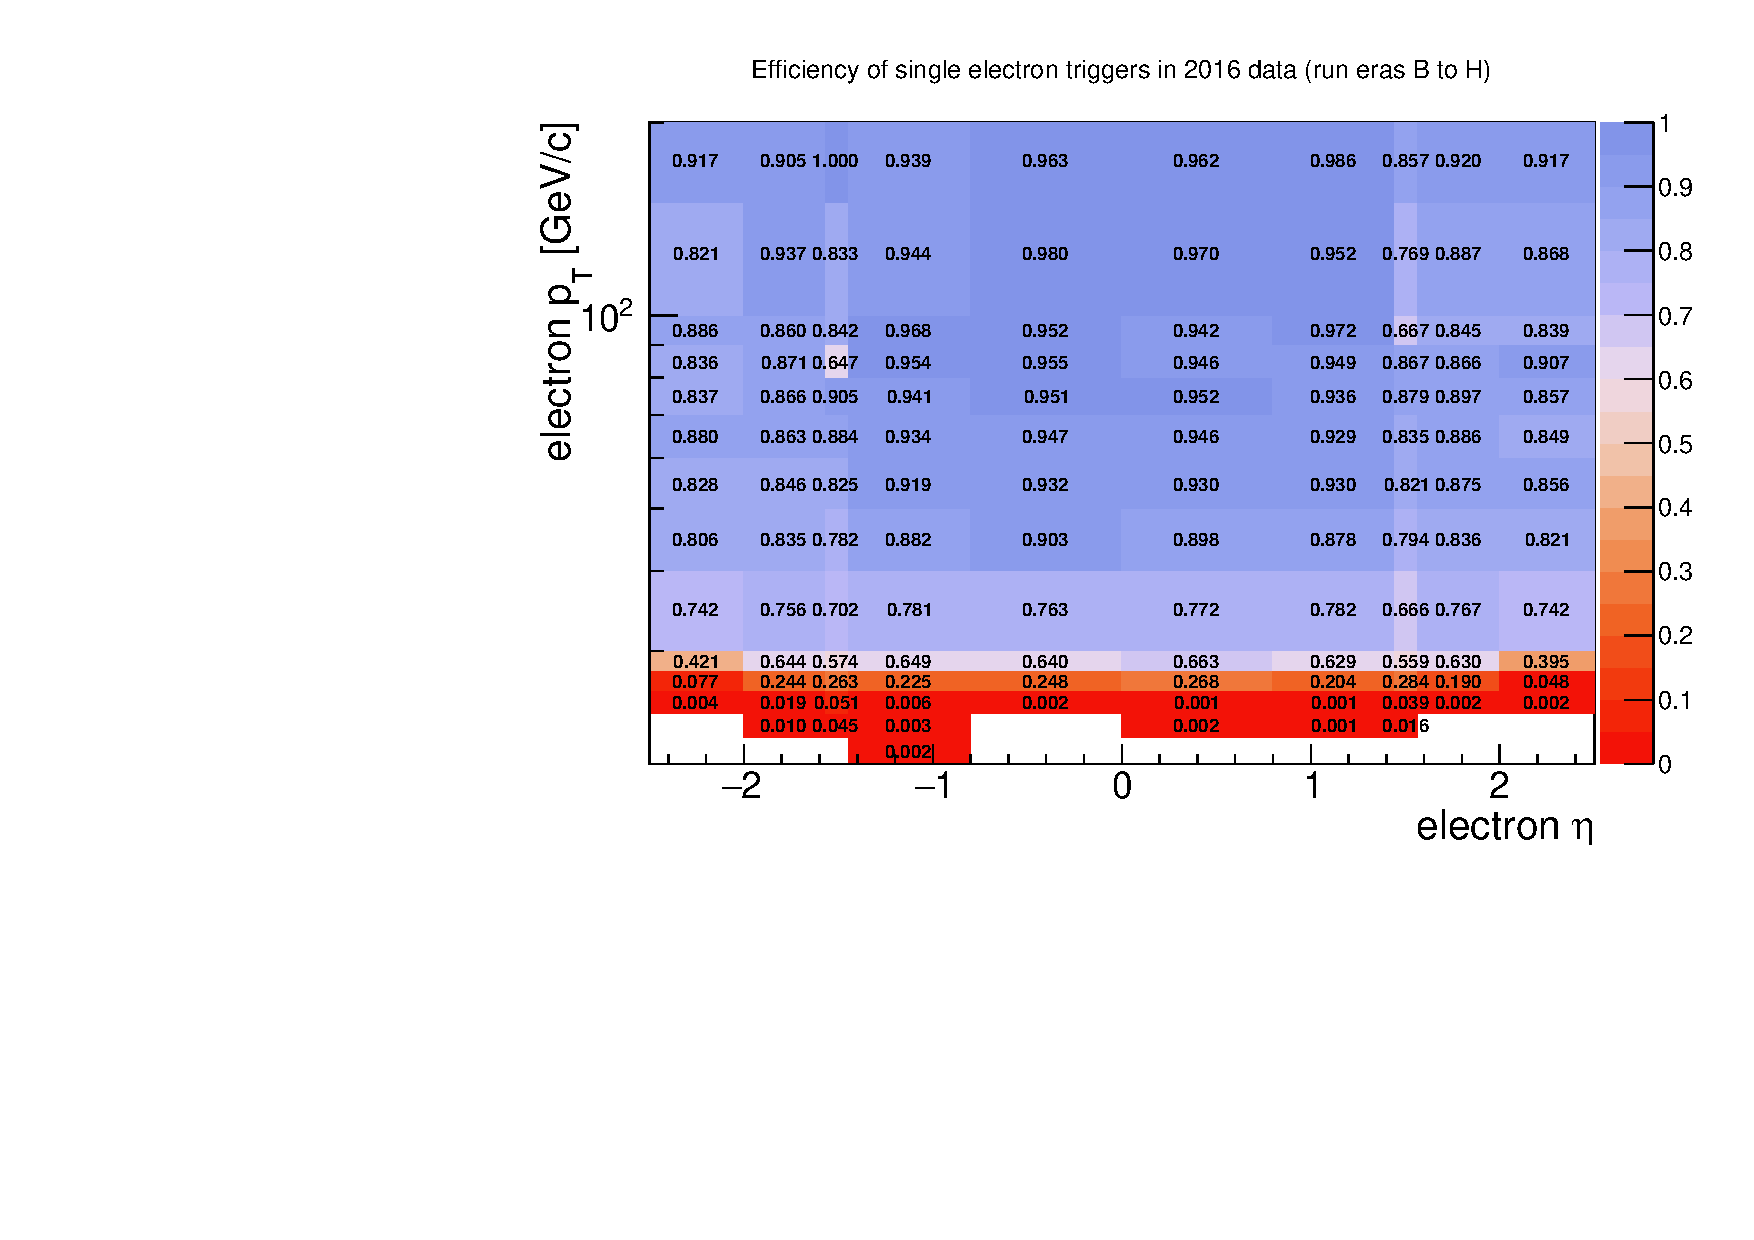
\includegraphics[width=0.75\textwidth]{figures/triggerstudies/singleElectronTrigger_Run2016BCDEFGH.pdf}
       \caption{Measured trigger efficiencies for the single electron triggers in 2016.}
 \label{fig:triggereffal}
 \end{center}
 \end{figure}
\begin{figure}[hbtp]\begin{center}
    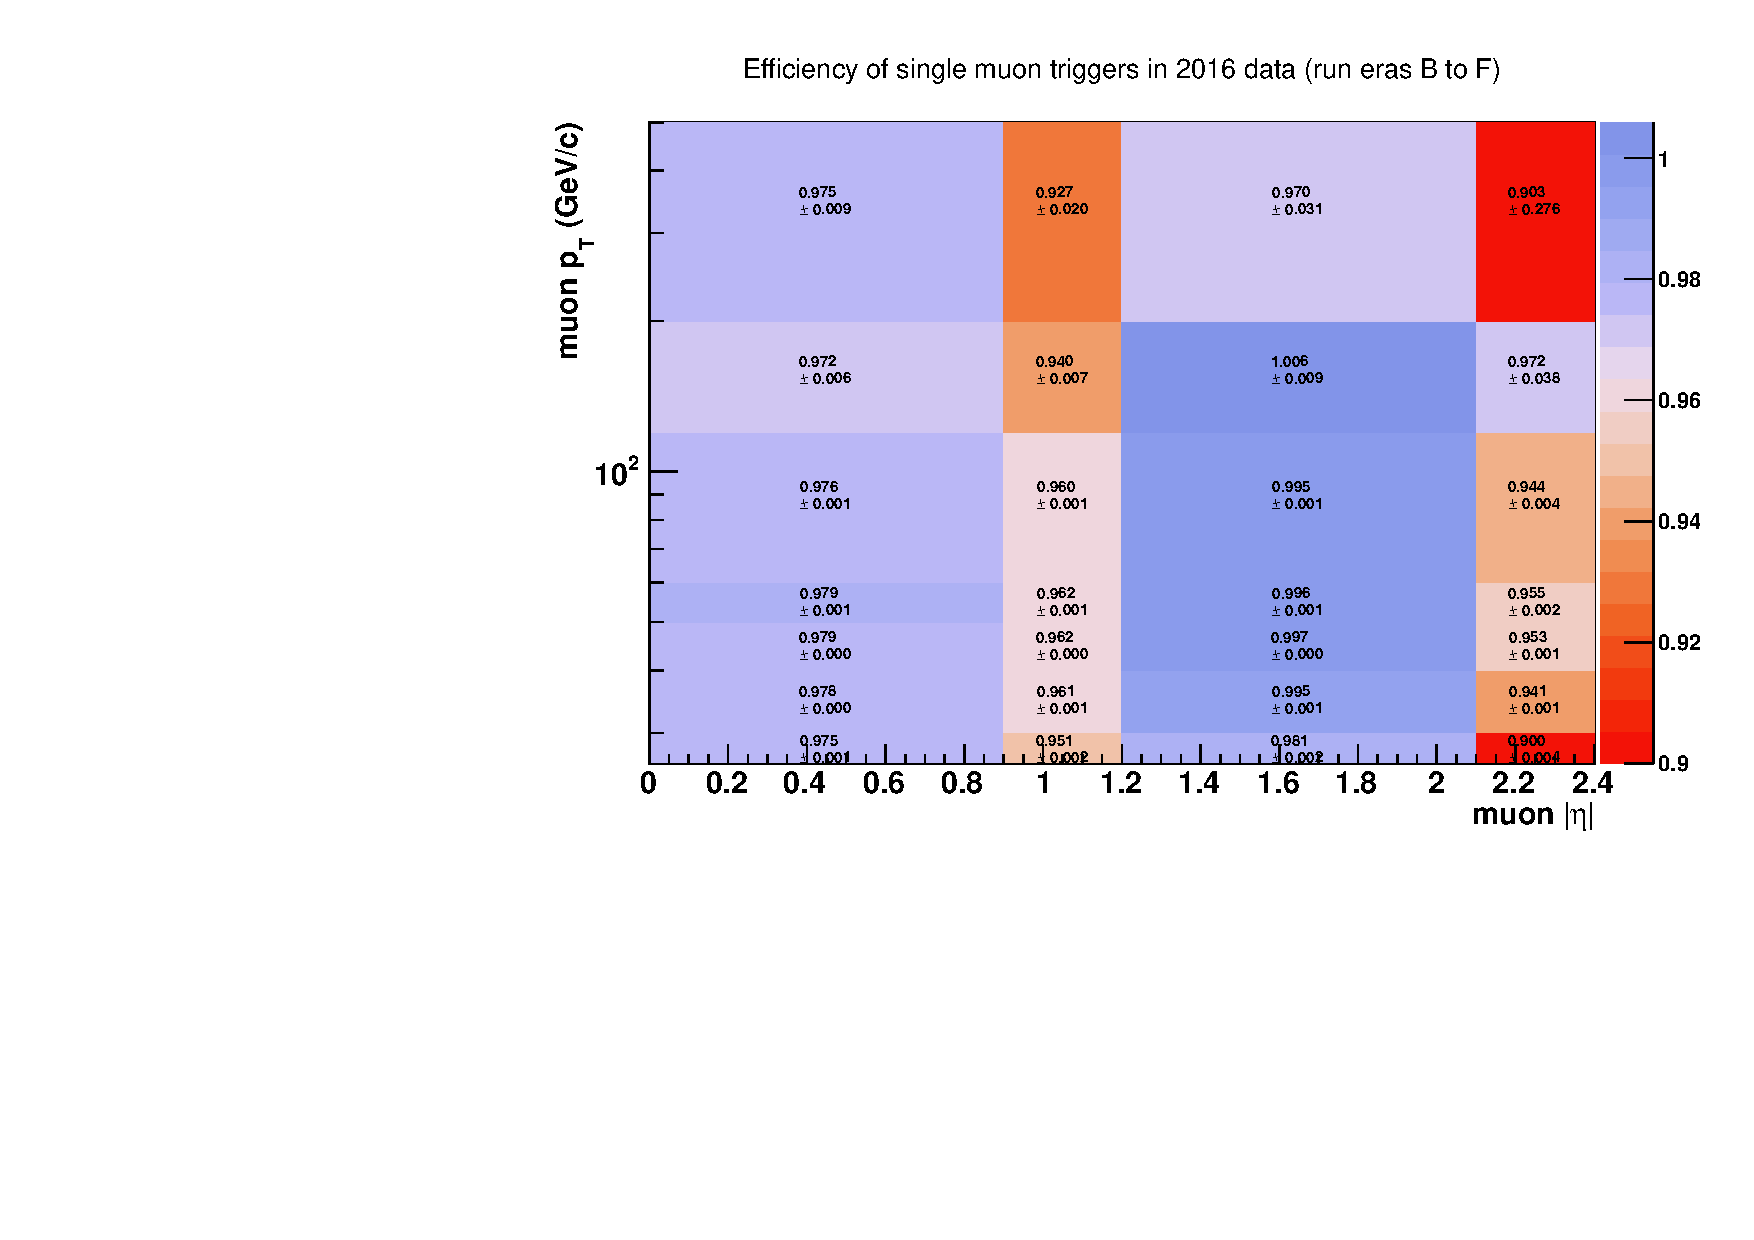
\includegraphics[width=0.75\textwidth]{figures/triggerstudies/singleMuonTrigger_Run2016BCDEF.pdf}
    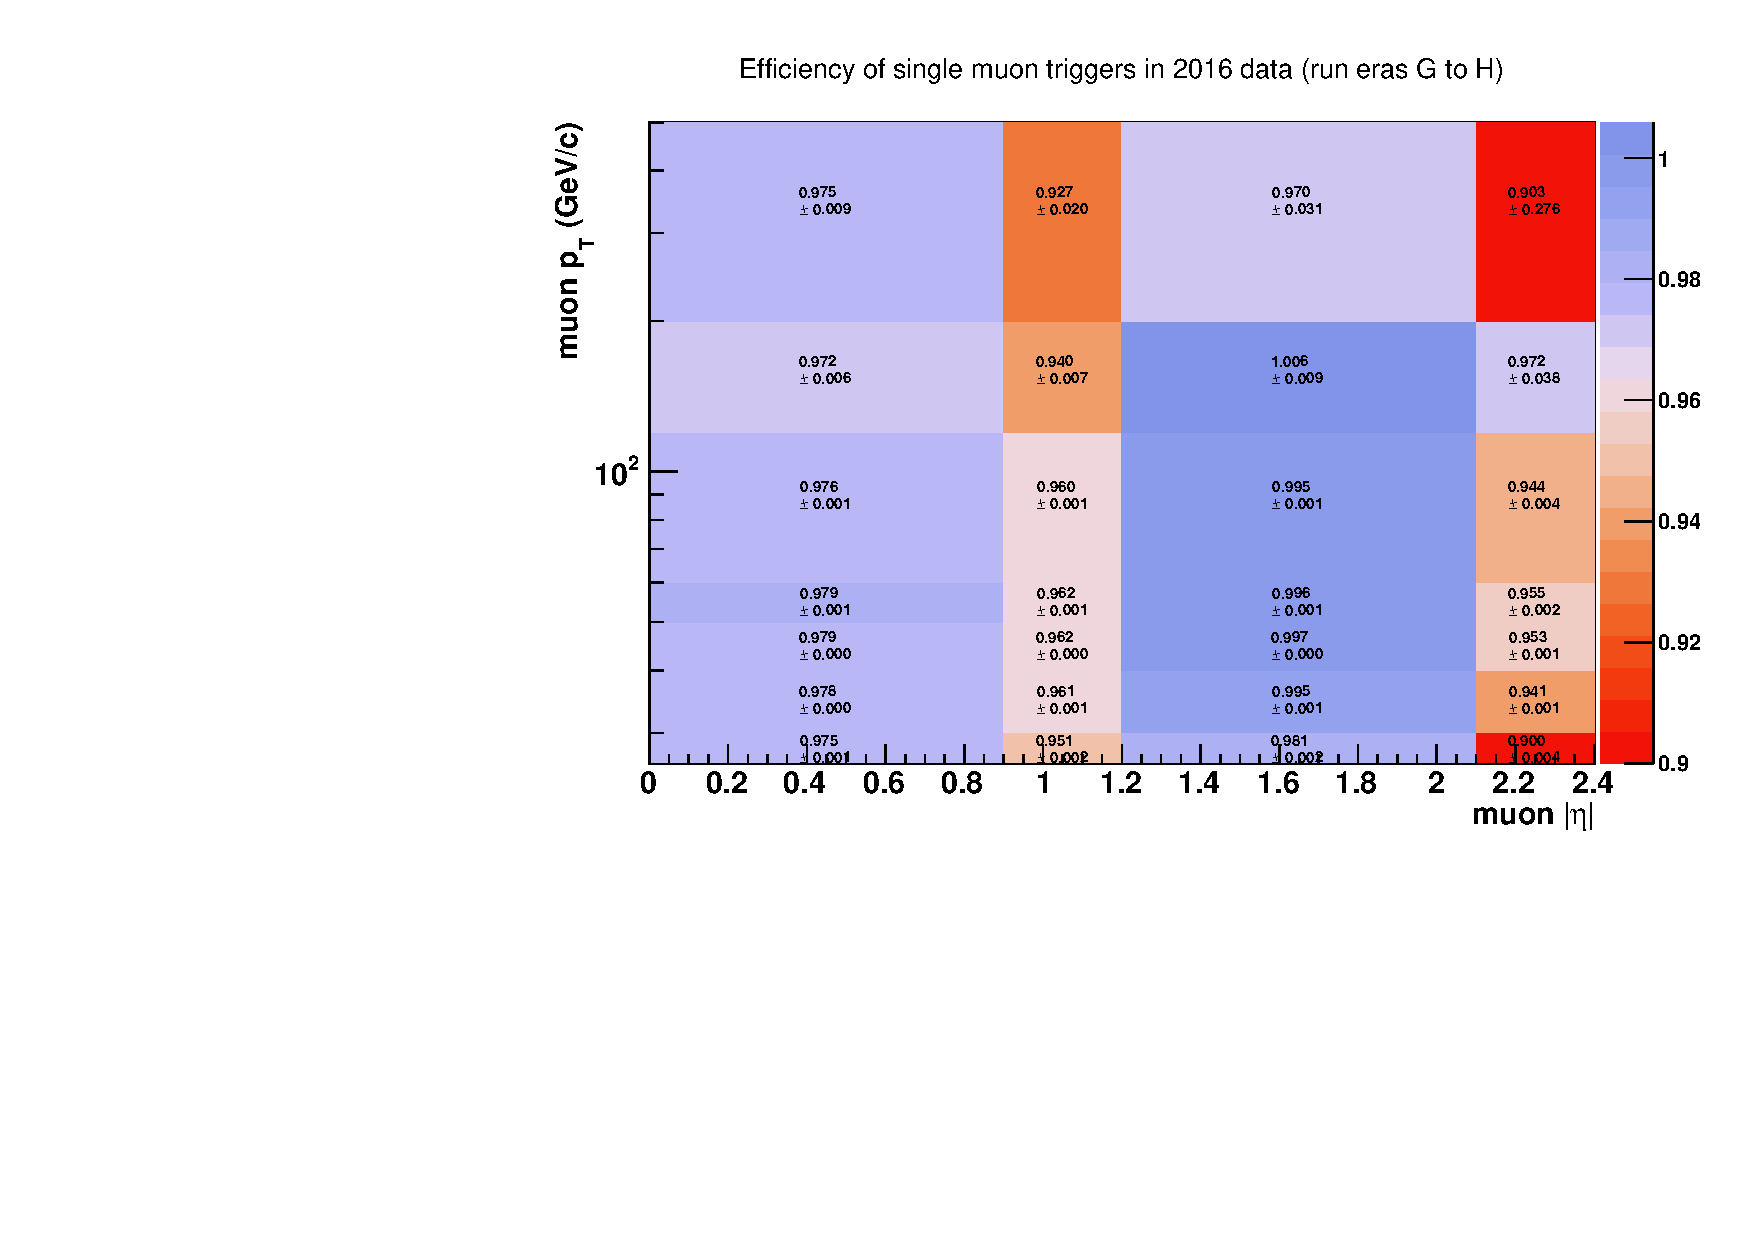
\includegraphics[width=0.75\textwidth]{figures/triggerstudies/singleMuonTrigger_Run2016GH.pdf}
       \caption{Measured trigger efficiencies for the single muon triggers in 2016.}
 \label{fig:triggereffal}
 \end{center}
 \end{figure}


\clearpage
\subsection{Monte-Carlo Simulation}
\label{sec:bkgsamples}

Monte~Carlo samples in CMSSW 80X are taken from the RunIISummer16  productions re-miniAODv2 with the {\it Asympt25ns} conditions. The Spring 2016 In-Time pileup scenario was used to approximate the number of inelastic collisions per bunch crossing at LHC 13 TeV data-taking. Appropriate event re-weighting is applied to reproduce the distribution of the number of primary vertexes in data. 

Samples were produced using one or more of the following programs:
\PYTHIA8~\cite{Sjostrand:2006za,Sjostrand:2007gs}, \POWHEG~\cite{Nason:2004rx}, \TAUOLA~\cite{Golonka:2003xt}, 
and \MADGRAPH5\_aMC@NLO~\cite{Alwall:2011uj,Alwall:2014hca}\
with {\sc MLM} merging~\cite{Mangano:2006rw} or FxFx merging scheme~\cite{Frederix:2012ps}.
Parton shower and hadronisation are performed with \PYTHIA8~\cite{Sjostrand:2007gs} using the CUETP8M1 tune~\cite{Khachatryan:2015pea}.
The {\sc NNPDF3.0} parton distribution functions (PDF)~\cite{Ball:2014uwa} are used for all samples.

The production cross sections for \PW+jets and Z+jets are rescaled to next-to-next-to-leading-order (NNLO)
cross sections calculated using the \FEWZ 3.1 program~\cite{Gavin:2010az,Li:2012wna,Gavin:2012sy}.
These corrections are binned in the generator-level scalar sum of parton $\pt$ (also known as LHE HT),
but we are thinking about ways to do this better.
The $\ttbar$ and single top quark samples are also rescaled to their cross sections based on
NNLO calculations~\cite{Czakon:2013goa, Kidonakis:2012db}.

The WZ and ZZ diboson processes are simulated at next-to-leading order in QCD
The continuum-induced ZZ contribution is neglected due to the small cross section.

The diboson MC samples are generated in electroweak leading-order. For the ZZ
background, a higher order electroweak correction is applied following~\cite{Bierweiler:2013dja,Gieseke:2014gka}  An event-by-event reweighting is performed with correction weights binned in the generator-level \pt of the trailing boson.
This correction results in a net reduction of the overall ZZ yield of about 10\%, although with a strong dependence on the trailing-boson $\pt$.
Overall, the $\pt$ spectrum becomes softer, with a correction of down to $-40\%$ for a trailing-Z $\pt$ of 700~$\GeV$. 
Following~\cite{Baglio:113005}, the corresponding NLO EWK correction to WZ production is small.

Furthermore, for the $\Pq\Pq \to $ZZ process, a QCD NLO to NNLO correction factor is
applied as a function of generator-level invariant mass of the two Z bosons~\cite{qqzz_kfactor,twiki:HZZ4LnnloZZ,talk:SperkaZZcorr}. 
In the case of the WZ process, a NLO to NNLO correction factor of 1.109 is applied~\cite{1604.08576}.

%A list of all background MC samples and the corresponding cross sections are given in Table~\ref{tab:bgmc}.  

\begin{table}[htbp]
\centering 
\resizebox{\textwidth}{!}{
  \begin{tabular}{l|c}
  \hline
  Dataset name & $\sigma$ [pb] \\
  \hline
  /DYJetsToLL\_M-50\_HT-100to200\_TuneCUETP8M1\_13TeV-madgraphMLM-pythia8        & 147.40   \\
  /DYJetsToLL\_M-50\_HT-200to400\_TuneCUETP8M1\_13TeV-madgraphMLM-pythia8        & 40.99    \\
  /DYJetsToLL\_M-50\_HT-400to600\_TuneCUETP8M1\_13TeV-madgraphMLM-pythia8        & 5.678    \\
  /DYJetsToLL\_M-50\_HT-600to800\_TuneCUETP8M1\_13TeV-madgraphMLM-pythia8        & 1.367    \\
  /DYJetsToLL\_M-50\_HT-800to1200\_TuneCUETP8M1\_13TeV-madgraphMLM-pythia8       & 0.6304   \\
  /DYJetsToLL\_M-50\_HT-1200to2500\_TuneCUETP8M1\_13TeV-madgraphMLM-pythia8      & 0.1514   \\
  /DYJetsToLL\_M-50\_HT-2500toInf\_TuneCUETP8M1\_13TeV-madgraphMLM-pythia8       & 0.003565 \\
  \hline
  /WJetsToLNu\_HT-100To200\_TuneCUETP8M1\_13TeV-madgraphMLM-pythia8              & 1343     \\ 
  /WJetsToLNu\_HT-200To400\_TuneCUETP8M1\_13TeV-madgraphMLM-pythia8              & 359.6    \\ 
  /WJetsToLNu\_HT-400To600\_TuneCUETP8M1\_13TeV-madgraphMLM-pythia8              & 48.85    \\ 
  /WJetsToLNu\_HT-600To800\_TuneCUETP8M1\_13TeV-madgraphMLM-pythia8              & 12.05    \\ 
  /WJetsToLNu\_HT-800To1200\_TuneCUETP8M1\_13TeV-madgraphMLM-pythia8             & 5.501    \\ 
  /WJetsToLNu\_HT-1200To2500\_TuneCUETP8M1\_13TeV-madgraphMLM-pythia8            & 1.329    \\ 
  /WJetsToLNu\_HT-2500ToInf\_TuneCUETP8M1\_13TeV-madgraphMLM-pythia8             & 0.03216  \\ 
  /WBJetsToLNu\_Wpt-100to200\_TuneCUETP8M1\_13TeV-madgraphMLM-pythia8            & 6.004    \\ 
  /WBJetsToLNu\_Wpt-200toInf\_TuneCUETP8M1\_13TeV-madgraphMLM-pythia8            & 0.8524   \\ 
  /WJetsToLNu\_BGenFilter\_Wpt-100to200\_TuneCUETP8M1\_13TeV-madgraphMLM-pythia8 & 71.77    \\ 
  /WJetsToLNu\_BGenFilter\_Wpt-200toInf\_TuneCUETP8M1\_13TeV-madgraphMLM-pythia8 & 3.027    \\ 
  \hline
  /ZJetsToNuNu\_HT-100To200\_13TeV-madgraph                                      & 280.5    \\ 
  /ZJetsToNuNu\_HT-200To400\_13TeV-madgraph                                      & 77.7     \\ 
  /ZJetsToNuNu\_HT-400To600\_13TeV-madgraph                                      & 10.71    \\ 
  /ZJetsToNuNu\_HT-600To800\_13TeV-madgraph                                      & 2.562    \\ 
  /ZJetsToNuNu\_HT-800To1200\_13TeV-madgraph                                     & 1.183    \\ 
  /ZJetsToNuNu\_HT-1200To2500\_13TeV-madgraph                                    & 0.286    \\ 
  /ZJetsToNuNu\_HT-2500ToInf\_13TeV-madgraph                                     & 0.006945 \\ 
  \hline
  \end{tabular}}
  \caption{List of background MC samples for the V+jets process. Datasets are LO in QCD and EWK, but will have NLO corrections applied.}
  %Cross-sections marked with $\dag$ are (N)NLO
  \label{tab:vjets_mc}
\end{table}

\begin{table}[htbp]
\centering 
\resizebox{\textwidth}{!}{
  \begin{tabular}{l|c}
  \hline
  Dataset name & $\sigma$ [pb] \\
  \hline
  /ST\_tW\_antitop\_5f\_inclusiveDecays\_13TeV-powheg-pythia8\_TuneCUETP8M1                  & 35.85    \\
  /ST\_tW\_top\_5f\_inclusiveDecays\_13TeV-powheg-pythia8\_TuneCUETP8M1                      & 35.85    \\
  /ST\_t-channel\_antitop\_4f\_inclusiveDecays\_13TeV-powhegV2-madspin-pythia8\_TuneCUETP8M1 & 80.95    \\
  /ST\_t-channel\_top\_4f\_inclusiveDecays\_13TeV-powhegV2-madspin-pythia8\_TuneCUETP8M1     & 136.02   \\
  \hline
  /TTTo2L2Nu\_TuneCUETP8M2\_ttHtranche3\_13TeV-powheg-pythia8                                & 88.288   \\
  /TT\_TuneCUETP8M2T4\_13TeV-powheg-pythia8                                                  & 831.76   \\
  \hline
  /QCD\_HT100to200\_TuneCUETP8M1\_13TeV-madgraphMLM-pythia8                                  & 27990000 \\  
  /QCD\_HT200to300\_TuneCUETP8M1\_13TeV-madgraphMLM-pythia8                                  & 1735000  \\  
  /QCD\_HT300to500\_TuneCUETP8M1\_13TeV-madgraphMLM-pythia8                                  & 366800   \\  
  /QCD\_HT500to700\_TuneCUETP8M1\_13TeV-madgraphMLM-pythia8                                  & 29370    \\  
  /QCD\_HT700to1000\_TuneCUETP8M1\_13TeV-madgraphMLM-pythia8                                 & 6524     \\  
  /QCD\_HT1000to1500\_TuneCUETP8M1\_13TeV-madgraphMLM-pythia8                                & 1064     \\  
  /QCD\_HT1500to2000\_TuneCUETP8M1\_13TeV-madgraphMLM-pythia8                                & 121.5    \\  
  /QCD\_HT2000toInf\_TuneCUETP8M1\_13TeV-madgraphMLM-pythia8                                 & 25.42    \\  
  \hline
  \end{tabular}}
  \caption{List of background MC samples for the top and QCD backgrounds.}
  %Cross-sections marked with $\dag$ are (N)NLO
  \label{tab:vjets_mc}
\end{table}

\begin{table}[htbp]
\centering 
\resizebox{\textwidth}{!}{
  \begin{tabular}{l|c}
  \hline
  Dataset name & $\sigma$ [pb] \\
  \hline
  /WWTo2L2Nu\_13TeV-powheg                             & 12.178  \\ 
  /WWTo4Q\_13TeV-powheg                                & 51.723  \\ 
  /WWToLNuQQ\_13TeV-powheg                             & 49.997  \\ 
  /WZTo1L1Nu2Q\_13TeV\_amcatnloFXFX\_madspin\_pythia8  & 10.71   \\   
  /WZTo1L3Nu\_13TeV\_amcatnloFXFX\_madspin\_pythia8    & 3.033   \\   
  /WZTo2L2Q\_13TeV\_amcatnloFXFX\_madspin\_pythia8     & 5.595   \\   
  /WZTo3LNu\_TuneCUETP8M1\_13TeV-powheg-pythia8        & 4.430   \\ 
  /ZZTo2L2Nu\_13TeV\_powheg\_pythia8                   & 0.5644  \\  
  /ZZTo2L2Q\_13TeV\_amcatnloFXFX\_madspin\_pythia8     & 3.22    \\   
  /ZZTo4L\_13TeV\_powheg\_pythia8                      & 1.212   \\  
  /ZZTo2Q2Nu\_13TeV\_amcatnloFXFX\_madspin\_pythia8    & 4.072   \\
  /ZZTo4Q\_13TeV\_amcatnloFXFX\_madspin\_pythia8       & 6.842   \\   
  \hline
  \end{tabular}}
  \caption{List of background MC samples for the diboson backgrounds. All samples that could have the VZ(bb) final state are simulated at NLO in QCD and LO in EWK, but will be corrected later.}
  %Cross-sections marked with $\dag$ are (N)NLO
  \label{tab:vjets_mc}
\end{table}
\begin{table}[htbp]
\centering 
\resizebox{\textwidth}{!}{
  \begin{tabular}{l|c}
  \hline
  Dataset name & $\sigma$ [pb] \\
  \hline
/WplusH\_HToBB\_WToLNu\_M125\_13TeV\_powheg\_pythia8   &  0.159  \\  
/WminusH\_HToBB\_WToLNu\_M125\_13TeV\_powheg\_pythia8  &  0.100  \\ 
  \hline
  \end{tabular}}
  \caption{List of signal MC samples. Cross sections are taken from the LHC Higgs Cross Section Working Group Yellow Report.}
  %Cross-sections marked with $\dag$ are (N)NLO
  \label{tab:signal_mc}
\end{table}

\subsubsection{\ttbar \pt corrections}
\label{sec:ttbarpt}
Correction factors are applied to the $\ttbar$ sample based on the $\pt$
re-weighting procedure recommended by the Top PAG and based on the
results of Ref.~\cite{CMS-PAS-TOP-16-011} and Ref.~\cite{Khachatryan:2016mnb}. The recommended
scale factor is~\cite{CMS-TOP-PT-REWEIGHT}
\begin{equation}
\mathrm{SF}(\pt) = e^{0.0615-0.0005\cdot \pt}~,
\end{equation}
with the overall event weight given by
$w=\sqrt{SF(\PQt)SF(\cPaqt)}$. The fit for the scale factor function is shown in
Fig.~\ref{fig:topPt}. 
\begin{figure}[hbtp]\begin{center}
    \includegraphics[width=0.45\textwidth]{figures/TopPt_DATA_PWHGP8.pdf}
    \caption{Top \pt reweighting function}
 \label{fig:topPt}
 \end{center}
 \end{figure}
